\chapter*{Appendix}\label{chap:app}
\addcontentsline{toc}{chapter}{Appendix}
\setcounter{section}{0}
\setcounter{figure}{0}
\renewcommand{\thesection}{\Alph{section}}
\renewcommand{\thesubsection}{\Alph{section}.\arabic{subsection}}
\numberwithin{figure}{section}
\renewcommand{\thefigure}{\Alph{section}.\arabic{figure}}

\vspace{-0.5cm}

\section{Big Bang Nucleosynthesis}

\subsection{Temperature Evolution and Universe's Expansion}\label{sec:evo}

When a neutrinophilic BSM particle is present, the differential equations governing the evolution of $T_\nu$ and $T_\gamma$ read:
\begin{subnumcases}{\hspace{-2.8cm}\textrm{Neutrinophilic }}
\label{eq:dTgamdt_DM_nu}
    \!\! \,\, \frac{dT_\nu}{dt} = -\frac{ 12 H \rho_\nu +3 H( \rho_{\chi} + p_{\chi})  - 3 \frac{\delta \rho_{\nu}}{\delta t}}{3 \, \frac{\partial \rho_\nu}{\partial T_\nu } +  \frac{\partial \rho_{\chi}}{\partial T_\nu } }\,, \\
    \!\! \,\, \frac{dT_{\gamma}}{dt}  =- \frac{  4 H \rho_{\gamma} + 3 H \left( \rho_{e} + p_{e}\right) + 3 H \, T_\gamma \frac{dP_{\text{int}}}{dT_\gamma}+3 \frac{\delta \rho_{\nu}}{\delta t}  }{ \frac{\partial \rho_{\gamma}}{\partial T_\gamma} + \frac{\partial \rho_e}{\partial T_\gamma} +T_\gamma \frac{d^2 P_{\text{int}}}{dT_\gamma^2} }\,,
\end{subnumcases}
whilst for an electrophilic particle, they are given by:
\begin{subnumcases}{\textrm{Electrophilic }}
    \!\! \,\, \frac{dT_\nu}{dt} = -\frac{ 12  H \rho_\nu  -  3 \frac{\delta \rho_{\nu}}{\delta t}}{3 \, \frac{\partial \rho_\nu}{\partial T_\nu }}\,, \\
    \!\! \,\, \frac{dT_{\gamma}}{dt}  =- \frac{  4 H \rho_{\gamma} + 3 H \left( \rho_{e} + p_{e}\right) +  3 H \left( \rho_{\chi} + p_{\chi}\right) + 3 H \, T_\gamma \frac{dP_{\text{int}}}{dT_\gamma}+ 3\frac{\delta \rho_{\nu}}{\delta t}  }{ \frac{\partial \rho_{\gamma}}{\partial T_\gamma} + \frac{\partial \rho_e}{\partial T_\gamma} + \frac{\partial \rho_{\chi}}{\partial T_\gamma} +T_\gamma \frac{d^2 P_{\text{int}}}{dT_\gamma^2} } \ , \label{eq:dTgamdt_DM_e}
\end{subnumcases}
where $\rho_i$ and $p_i$ correspond to the energy density and pressure of a given particle respectively, $H = \sqrt{(8\pi/3)\,\sum_i \rho_i/M_{\rm Pl}^2}$ is the Hubble parameter, $M_{\rm Pl} = 1.22\times 10^{19}\,\text{GeV}$ the Planck mass, and $P_{\rm int}$ and its derivatives account for finite temperature corrections. The reader is referred to~\cite{Escudero:2018mvt} for further details. Here, $\delta \rho_{\nu} /\delta t$ corresponds to the energy exchange rate between neutrinos and electrons. Accounting for Fermi-Dirac statistics in the rates and setting $m_e = 0$, it reads~\cite{Escudero:2019new}:
\begin{align}\label{eq:energyrates_nu_SM}
& \left. \frac{\delta \rho_{\nu}}{\delta t}  \right|_{\rm SM} = \frac{G_F^2}{\pi^5} \left( 1 - \frac{4}{3} s_W^2 + 8 s_W^4 \right) \times  \left[ 32 \, f_a^{\rm FD} \,  \left( T_\gamma^9-T_{\nu}^9  \right) +  56 \,f_s^{\rm FD} \,   T_\gamma^4 \, T_{\nu}^4 \, \left( T_\gamma - T_{\nu}\right)\right] \,,
\end{align}
where $s_{\mathrm{W}}^2 = 0.223$~\cite{pdg}, $G_{\mathrm{F}}$ is Fermi's constant, $f_a^{\rm FD} = 0.884$, $f_s^{\rm FD} = 0.829$, and we account for the electron mass as in~\cite{Escudero:2019new}. 

We solve Equations~\eqref{eq:dTgamdt_DM_nu} -- \eqref{eq:dTgamdt_DM_e} for $1\,\text{keV} < T_\gamma < 30\,\text{MeV}$. We start the integration at $t_0 = 1/(2 H)|_{T = 30\,\text{MeV}}$ for which we use as an initial condition $T_\gamma = T_\nu = 30 \,\text{MeV}$, since for such high temperatures SM neutrino-electron interactions are highly efficient. By solving this set of differential equations, we find all the key background evolution quantities as a function of time, scale factor and temperature. In addition, we evaluate the number of effective relativistic degrees of freedom $N_{\rm eff}$ as relevant for CMB observations,
\begin{align}\label{eq:Neff}
N_{\rm eff} \equiv \frac{8}{7}\left(\frac{11}{4} \right)^{4/3} \left( \frac{\rho_{\text{rad}}-\rho_\gamma}{\rho_\gamma}\right) = 3 \left(\frac{11}{4} \right)^{4/3} \left(\frac{T_\nu}{T_\gamma}\right)^4 \, ,
\end{align} 
where in the last step we have assumed that $\rho_{\text{rad}} = \rho_\nu + \rho_\gamma$. By solving this system of equations in the SM we find $N_{\rm eff}^{\rm SM} = 3.046$~\cite{Escudero:2019new}, a result that is in perfect agreement with state-of-the-art calculations~\cite{Mangano:2005cc,deSalas:2016ztq}.  

\subsection{Consistency Checks of Modified BBN Code}\label{app:ConsistencyChecks}\vspace{-0.2cm}
%%%%%%%%%%%%%%%%%%%%%%%%%%%%%%%%%%%%%%%%%%%%%%%%%%%%%%
We checked whether our modifications do not significantly change the values of the primordial helium and deuterium abundances in Standard Model BBN compared to the base version of \texttt{PRIMAT}. Table \ref{tab:SBBNcheck} shows the relative difference in the output of the two codes and it is clear that the accuracy is better than $0.1\%$.
\begin{table}[h]
    \centering
    {\def\arraystretch{1.35}
    \begin{tabular}{c|c|c|c}
        \toprule
      $\,\,$   \textbf{Abundances} $\,\,$ & $\,\,$ \texttt{PRIMAT}$\,\,$ & $\,\,$ \textbf{Modified} \texttt{PRIMAT} $\,\,$ & $\,\,$ \textbf{Relative Difference (\%)} $\,\,$ \\
        \hline\hline
        $Y_{\mathrm{p}}$ & 0.24709 & 0.24717 & 0.03\\
        $10^5\times {\rm D/H}|_{\rm P}$ & 2.4592 & 2.4613 & 0.08 \\ \hline  \hline
    \end{tabular}}\vspace{-0.1cm}
    \caption{Primordial abundances as computed using \texttt{PRIMAT} and our modified version with $\Omega_{\mathrm{b}} h^2 = 0.02225$ and $\tau_n = 879.5$ s.}
    \label{tab:SBBNcheck}
\end{table} 
\vspace{-0.5cm}

\begin{figure}[t]
    \centering
    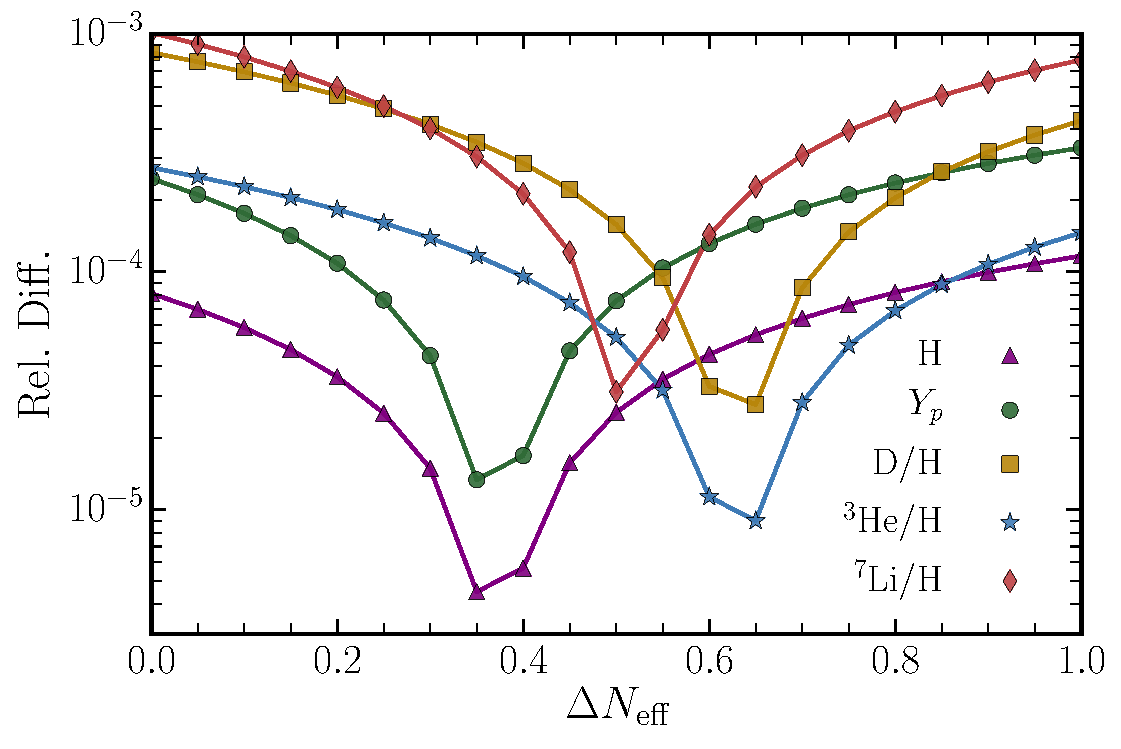
\includegraphics[width=0.5\textwidth]{figures/Neffcheck.pdf}\vspace{-0.5cm}
    \caption{Relative difference in the primordial abundances between the default version of \texttt{PRIMAT} and our modified version of it as a function of $\Delta N_{\mathrm{eff}}$. Predictions are done using $\Omega_{\mathrm{b}} h^2 = 0.02225$ and $\tau_n = 879.5$ s.}
    \label{fig:CheckDeltaNeff}
\end{figure}

\noindent We also compared our modifications to \texttt{PRIMAT} when massless dark radiation is present, which we parametrize in terms of $\Delta N_{\rm eff}$. In \texttt{PRIMAT} this is done by increasing $N_{\mathrm{eff}}$ directly in the Friedmann equations while in our modified version of the code it is done by including the evolution of a non-interacting, relativistic component. The result is shown in Figure \ref{fig:CheckDeltaNeff}.
The test shows an accuracy better than $0.1\%$ for all relevant nuclides in the range $0 \leq \Delta N_{\rm eff} \leq 1$.

\begin{figure*}[t]
    \begin{center}
    \begin{tabular}{cc}
     \hspace{-0.5cm} 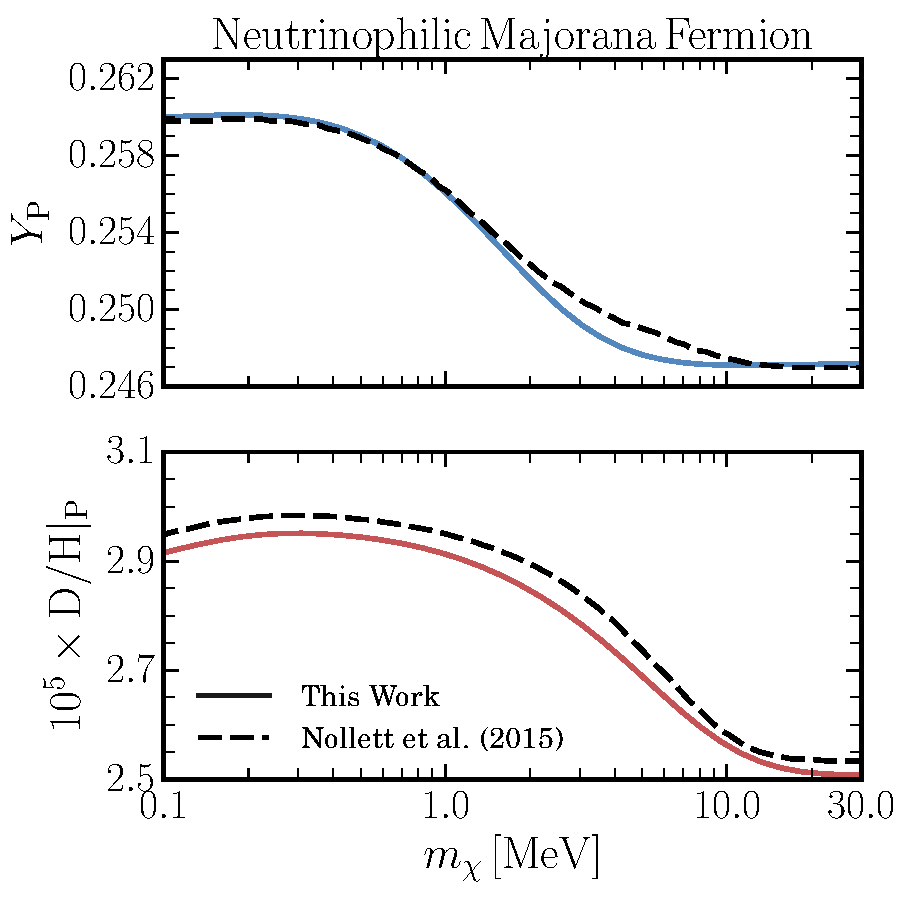
\includegraphics[width=0.46\textwidth]{figures/NollettNU.pdf}  \hspace{0.4cm} 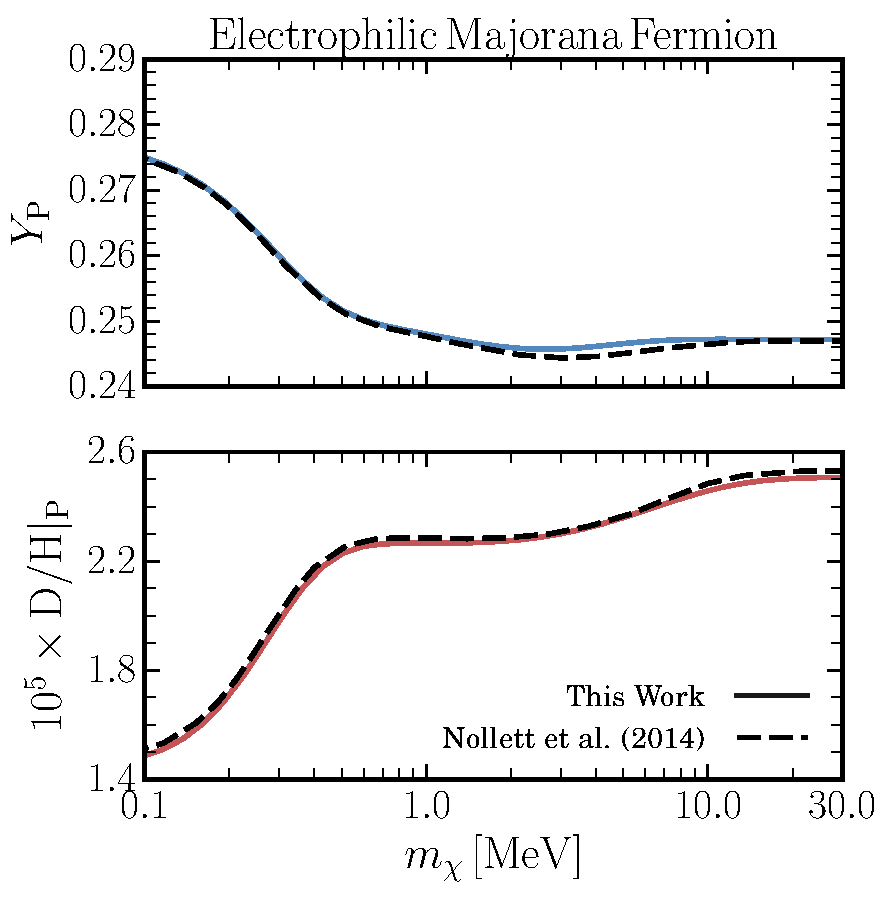
\includegraphics[width=0.45\textwidth]{figures/NollettEE.pdf}
      \end{tabular}
      \end{center}\vspace{-0.8cm}
    \caption{Comparison with previous literature for the primordial abundances $Y_{\mathrm{P}}$ and $\mathrm{D}/\mathrm{H}|_{\mathrm{P}}$ as a function of the mass of a Majorana BSM particle that couples exclusively to neutrinos (left panels) or electrons (right panels). The solid lines are from this work and the dashed lines from ~\cite{Nollett:2013pwa} and~\cite{Nollett:2014lwa}.}
    \label{fig:mccabe}
    \vspace{-0.5cm}
\end{figure*}

\subsection{Comparison with Previous Literature}\vspace{-0.2cm} \label{app:ComparisonsLiterature}
%%%%%%%%%%%%%%%%%%%%%%%%%%%%%%%%%%%%%%%%%%%%%%%%%%%%%%
In this appendix we make a direct comparison between our results and those reported in~\cite{Nollett:2013pwa} and~\cite{Nollett:2014lwa}. Refs~\cite{Nollett:2013pwa} and~\cite{Nollett:2014lwa} used a modified version of the Kawano code~\cite{Kawano:1988vh,Kawano:1992ua}. In Figure \ref{fig:mccabe}, we consider two cases: a Majorana fermion that is purely neutrinophilic or electrophilic. We compute the predictions for helium and deuterium using $\tau_{\mathrm{n}} =  880.1$ s and $\Omega_{\mathrm{b}}h^2 = 0.022 $ as in~\cite{Nollett:2013pwa} and~\cite{Nollett:2014lwa}. We observe a few small differences:
\begin{enumerate}[leftmargin=0.5cm,itemsep=0pt]\vspace{-0.1cm}
    \item Our predicted values of $\mathrm{D}/\mathrm{H}|_{\mathrm{P}}$ are smaller than those reported in~\cite{Nollett:2013pwa,Nollett:2014lwa}. Since the difference is WIMP mass independent, we attribute it to updated nuclear reaction rates in \texttt{PRIMAT}. 
    \item The predicted values of $Y_{\mathrm{P}}$ are slightly different for $ 1 \,\text{MeV} \lesssim   m_{\chi} \lesssim 15 \,\text{MeV}$. The reason is twofold:
    \begin{enumerate}[leftmargin=0.5cm,itemsep=0pt]\vspace{-0.1cm}
    \item \cite{Nollett:2013pwa,Nollett:2014lwa} considered that neutrinos decoupled instantaneously and tracked the temperature evolution by using entropy conservation, while we solve for the time evolution of neutrino decoupling. Imposing entropy conservation leads to a feature in the neutrino temperature evolution that affects both the Universe's expansion and the proton-to-neutron conversion rates, see Figure 2 of \cite{Escudero:2018mvt}.
    \item \cite{Nollett:2013pwa,Nollett:2014lwa} considered instantaneous neutrino decoupling at $T_\nu^{\rm dec} = 2.0\,\text{MeV}$, while an estimate based on the actual neutrino temperature time evolution yields $T_\nu^{\rm dec} = 1.91\,\text{MeV}$ \cite{Escudero:2018mvt}. Considering a smaller neutrino decoupling temperature leads to an impact on the proton-to-neutron rates and also reduces the impact of heavier BSM species in neutrino decoupling. 
    \end{enumerate}
\end{enumerate}\vspace{-0.1cm}
We have also compared our predictions of $Y_{\mathrm{P}}$ and $\mathrm{D}/\mathrm{H}|_{\mathrm{P}}$ with those reported in~\cite{Boehm:2013jpa} (which used  \texttt{PArthENoPEv1} \cite{Pisanti:2007hk}, see \cite{Consiglio:2017pot} for an updated version of the code). We find good overall agreement with~\cite{Boehm:2013jpa} and small differences similar to those we find when comparing to~\cite{Nollett:2013pwa,Nollett:2014lwa}. Note that~\cite{Wilkinson:2016gsy} provided updated bounds to those presented in~\cite{Boehm:2013jpa} although the predictions for $Y_{\mathrm{P}}$ and $\mathrm{D}/\mathrm{H}|_{\mathrm{P}}$ are not displayed in that reference.

%%%%%%%%%%%%%%%%%%%%%%%%%%%%%%%%%%%%%%%%%%%%%%%%%%%%%%
\subsection{Conservative Range for the Baryon Density from CMB observations} \label{app:Omegab}
%%%%%%%%%%%%%%%%%%%%%%%%%%%%%%%%%%%%%%%%%%%%%%%%%%%%%%

In the BBN+$\Omega_{\rm b}h^2$ analysis we consider $\Omega_{\mathrm{b}} h^2 = 0.02225 \pm 0.00066$ to be a conservative and cosmological model independent determination of the baryon energy density by current CMB observations. $\Omega_{\mathrm{b}} h^2 = 0.02225 \pm 0.00066$ has a $4.4$ times larger error bar than the one associated with $\Lambda\text{CDM}$ using Planck 2018 observations~\cite{Aghanim:2018eyx}, and furthermore, it covers well the inferred value of $\Omega_{\mathrm{b}} h^2$ in a well-motivated 12-parameter extensions of $\Lambda$CDM using different data sets~\cite{DiValentino:2016hlg,DiValentino:2017zyq}. In Figure \ref{fig:omegab}, one can appreciate that indeed the range with a central value of $\Omega_{\mathrm{b}} h^2 = 0.02225 \pm 0.00066$ covers very well the posterior distributions of $\Omega_{\mathrm{b}} h^2 $ of such a 12-parameter extension of $\Lambda$CDM including various data sets in conjuntion to Planck CMB observations. 

\begin{figure}[t]
    \centering
    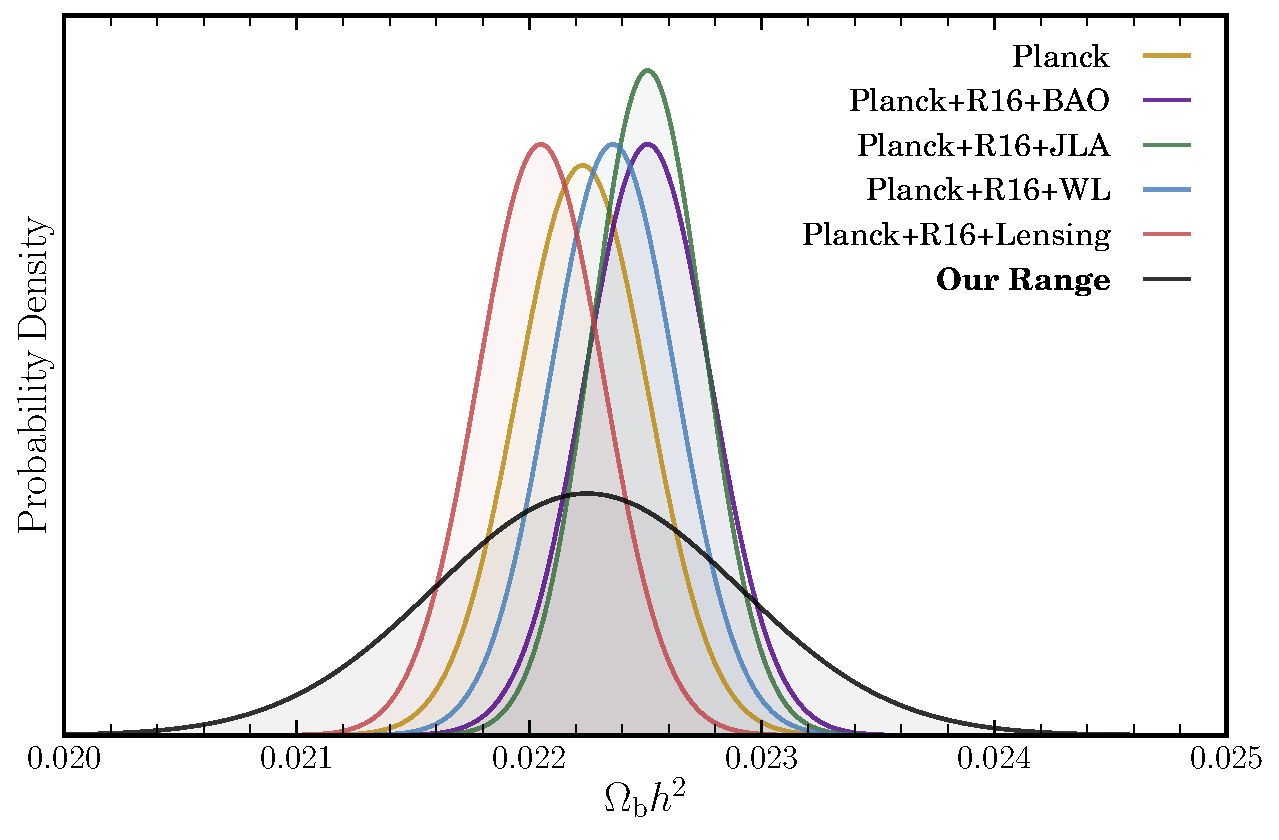
\includegraphics[width=0.6\textwidth]{figures/omegabposteriors.pdf}\vspace{-0.3cm}
    \caption{Illustration of the parameter range for the baryon density we consider in the BBN+$\Omega_{\mathrm{b}}h^2$ analysis as compared to the best-fit values and errors given in Table II of \cite{DiValentino:2017zyq}. The authors of \cite{DiValentino:2017zyq} infer $\Omega_{\mathrm{b}}h^2$ in a well-motivated 12-parameter extension to $\Lambda$CDM using the different data sets shown in the legend. Note in particular that our conservative range for the baryon density encompasses all derived central values and errors.}
    \label{fig:omegab}
\end{figure}
%%%%%%%%%%%%%%%%%%%%%%%%%%%%%%%%%%%%%%%%%%%%%%%%%%%%%%
\subsection{Implications for Lithium-7 and Helium-3}
\label{app:cosmo_imp_other}
We show the evolution of the primordial $^7\mathrm{Li}/\mathrm{H}|_{\mathrm{P}}$ and $^3\mathrm{He}/\mathrm{H}|_{\mathrm{P}}$ abundances in Figure \ref{fig:Cosmoimply_other} as a function of the mass of a thermal BSM particle. We note that the upper panels do not include any confidence intervals, since it is well known that current measurements of the primordial lithium-7 are in disagreement with SM predictions using the baryon-to-photon ratio inferred from CMB observations \cite{pdg}. The excluded regions in the lower panels are based on observations of helium-3 in our galaxy \cite{Bania:2002yj}. Helium-3 can be both produced and destroyed in stars, which makes it difficult to precisely determine the time evolution of its primordial abundance \cite{VangioniFlam:2002sa}. Therefore, we have not included measurements of either lithium-7 or helium-3 in our analysis. Nevertheless, if the situation changes in the future, it will be straightforward to obtain bounds from Figure \ref{fig:Cosmoimply_other} and see how it improves the current BBN constraints.
\clearpage

\begin{figure}[!ht]
    \centering
    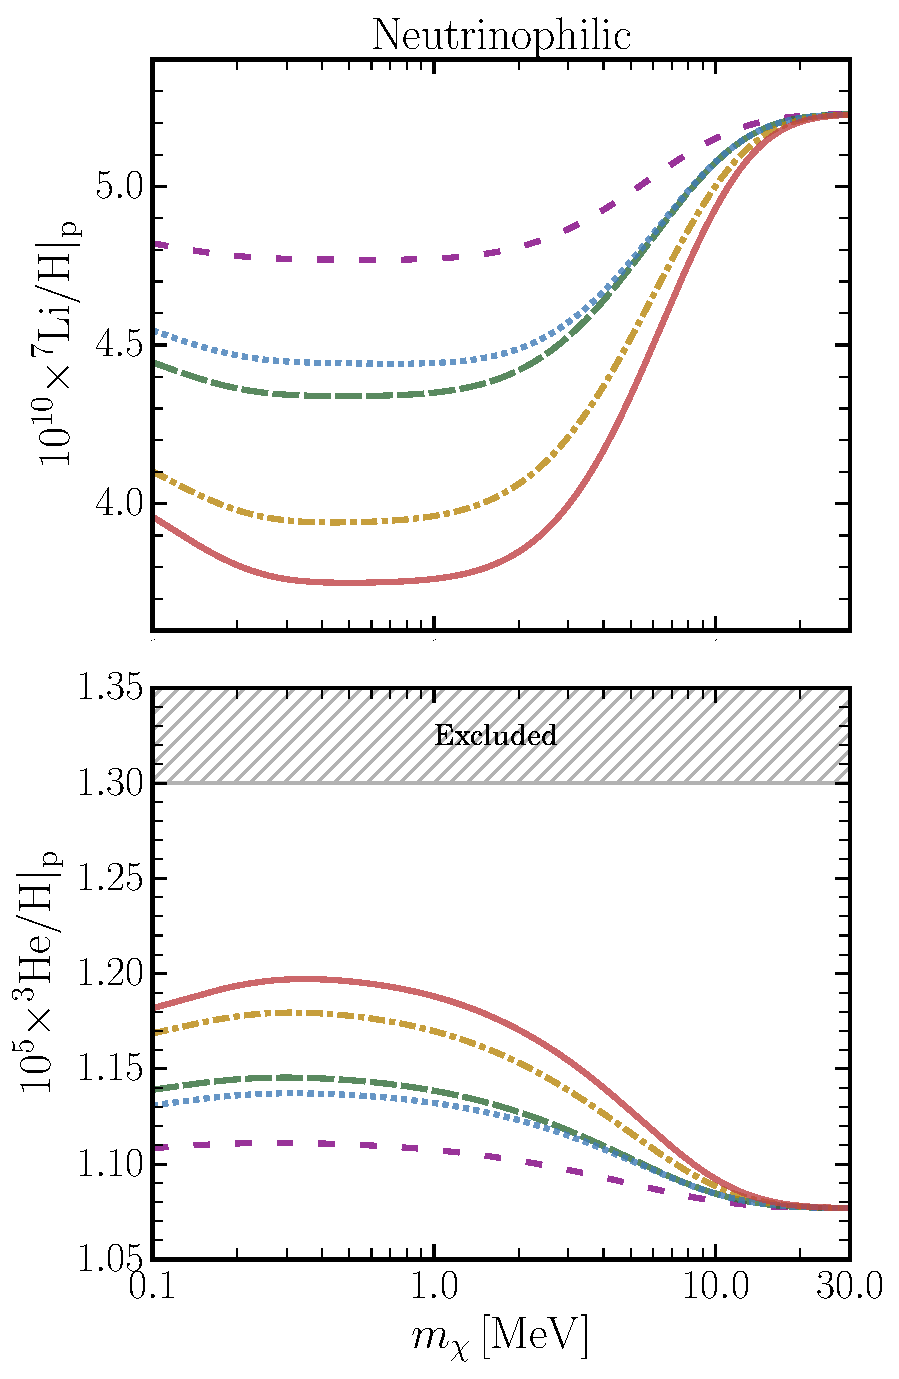
\includegraphics[width=0.46\textwidth]{figures/Nu_extra_abundance_plot.pdf} \qquad
    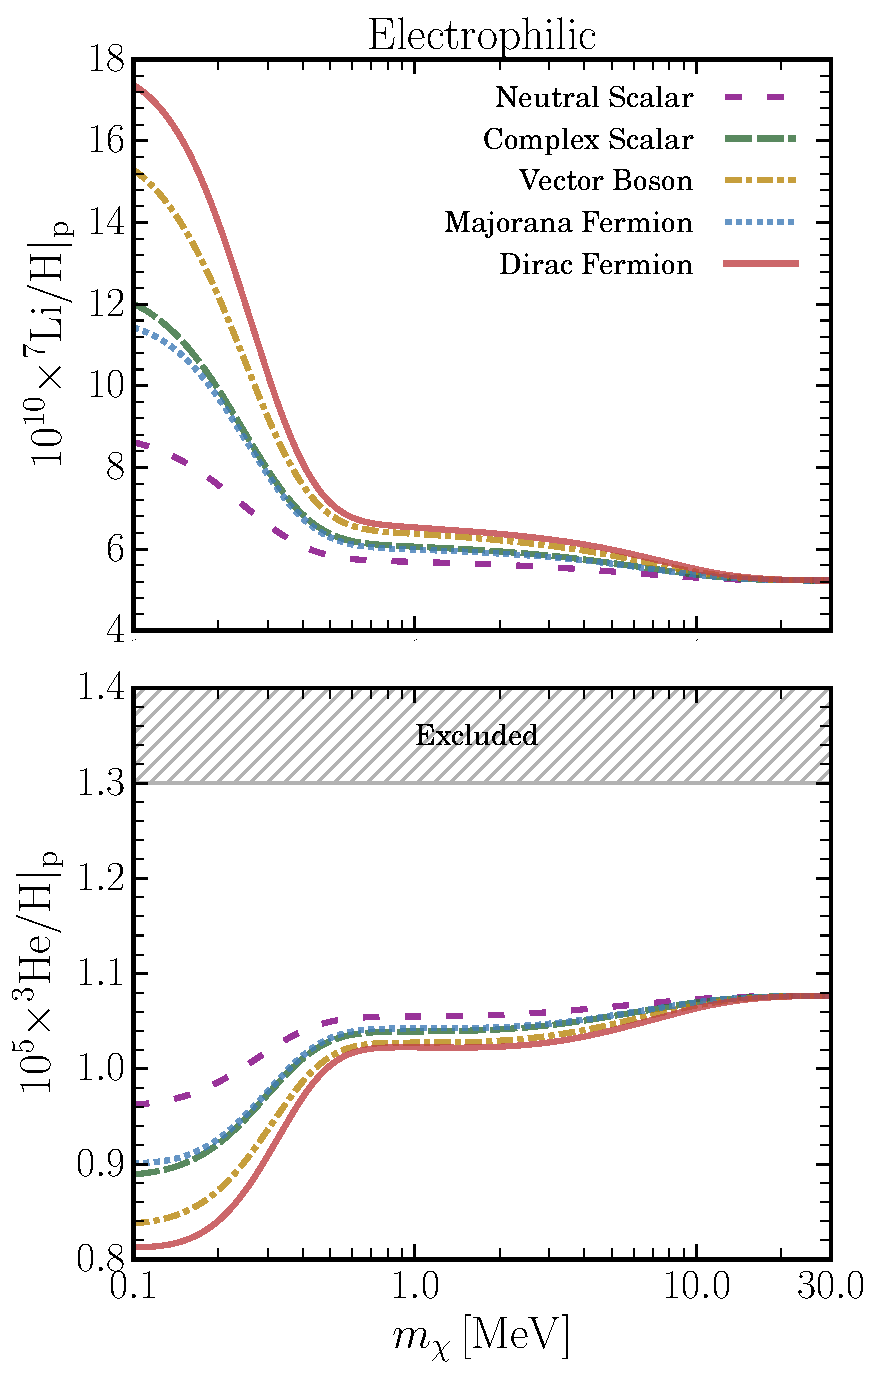
\includegraphics[width=0.45\textwidth]{figures/EE_extra_abundance_plot.pdf}
    \caption{Cosmological impact of light BSM particles in thermal equilibrium with the SM plasma as a function of their mass $m_\chi$. The \textit{left/right panels} correspond to neutrinophilic/electrophilic particles. \textit{Upper panels:} The lithium-7 primordial abundance $^7\mathrm{Li}/\mathrm{H}|_{\mathrm{P}}$. Measurements of $^7\mathrm{Li}/\mathrm{H}|_{\mathrm{P}}$ are not shown for clarity, see e.g. \cite{pdg} for current measurements. \textit{Lower panels:} The helium-3 primordial abundance $^3\mathrm{He}/\mathrm{H}|_{\mathrm{P}}$. The grey contours correspond to an upper limit as reported by~\cite{Bania:2002yj}. The predictions are made with $\Omega_{\mathrm{b}} h^2 = 0.021875$ and $\tau_n = 879.5\,\text{s}$.}
    \label{fig:Cosmoimply_other}
\end{figure}

\subsection{CMB-S4 Forecast}
\label{app:CMBfisher}
%%%%%%%%%%%%%%%%%%%%%%%%%%%%%%%%%%%%%%%%%%%%%%%%%%%%%%
In order to forecast the reach of CMB-S4 constraints, we first choose a fiducial cosmology with cosmological parameters equal to the Planck 2018 TTTEEE+lowE mean values as in Table 2 of \cite{Aghanim:2018eyx}, which are reproduced below in Table \ref{tab:FisherResults}.
The fiducial helium abundance is obtained by running \texttt{PRIMAT} within the Standard Model and fiducial cosmology.\\\\
\noindent To forecast the sensitivity of future CMB experiments, we employ the same procedure as used in the CMB-S4 Science Book \cite{Abazajian:2016yjj}. Assuming Gaussian statistics, the Fisher matrix for CMB experiments is given by
\begin{equation}
F_{i j}=\sum_{X, Y} \sum_{\ell=\ell_{\min }}^{\ell_{\max }} \frac{\partial \mathcal{C}_{\ell}^{X}}{\partial \theta_{i}}\left[\mathbf{C}_{\ell}^{X Y}\right]^{-1} \frac{\partial \mathcal{C}_{\ell}^{Y}}{\partial \theta_{i}}
\end{equation}
with indices $X = ab$, $Y = cd$ and $a,b,c,d\in\{T,E,B\}$. 
The covariance matrix $\mathbf{C}_\ell^{XY}$ for each multipole $\ell$ is defined as
\begin{align}
    \mathbf{C}_\ell^{abcd} =& \frac{1}{(2\ell+1)f_{\mathrm{sky}}}\left[\left(\mathcal{C}_\ell^{ac}+N_\ell^{ac}\right)\left(\mathcal{C}_\ell^{bd}+N_\ell^{bd}\right)
    + \left(\mathcal{C}_\ell^{ad}+N_\ell^{ad}\right)\left(\mathcal{C}_\ell^{bc}+N_\ell^{bc}\right)\right]\ ,
\end{align}
with $f_{\mathrm{sky}}$ the effective fraction of sky covered by the experiment, $\mathcal{C}_\ell^X$ the simulated CMB power spectra and $N_\ell^X$ (Gaussian) noise power spectra. The noise is approximated as
\begin{align}
    N_\ell^{aa} = (\Delta X)^2\exp\left(\frac{\ell(\ell+1)\theta^2_{\mathrm{FWHM}}}{8\ln2}\right)\ ,
\end{align}
where $\Delta X \in \{\Delta T,\Delta P\}$ and $N_\ell^{TE} = 0$.
We adopt a similar configuration as used in the CMB-S4 Science Book: lensed power spectra with $\ell_{\mathrm{min}} = 30$, $\{\ell_{\mathrm{max}}^{TT}, \ell_{\mathrm{max}}^{TE}\} = 3000$, $\{\ell_{\mathrm{max}}^{EE},\ell_{\mathrm{max}}^{BB}\} = 5000$, $f_{\mathrm{sky}} = 0.4$, $\theta_{\mathrm{FWHM}} = 1'$, $\Delta T = 1$ $\mu$K-arcmin and $\Delta P = \sqrt{2}$ $\mu$K-arcmin.\\\\
The \texttt{CLASS} code \cite{Blas:2011rf} is used to obtain the power spectra. The numerical derivatives are computed using the symmetric derivative $\mathcal{C}_\ell'(\theta) = \left[\mathcal{C}_\ell(\theta+\Delta\theta)-\mathcal{C}_\ell(\theta-\Delta\theta)\right]/(2\Delta\theta)$, with fiducial parameter $\theta$ and stepsize $\Delta\theta$. The stepsizes used are of order $\Delta\theta_i \sim \sigma(\theta_i)$, as to output a more reliable estimate of the confidence level \cite{Perotto:2006rj}. The CMB-S4 Fisher matrix is then added to the Planck 2018 low-$\ell$ TTTEEE+lowP+lowE Fisher matrix to obtain the combined constraints. The fiducial parameters and step sizes used in our computations, together with the forecasted sensitivities, are listed in Table \ref{tab:FisherResults}. We find good overall agreement with the forecasts performed in \cite{Abazajian:2016yjj} within $\Lambda$CDM. 

\begin{table}[!ht]
\begin{center}
{\def\arraystretch{1.35}
\resizebox{\textwidth}{!}{
\begin{tabular}{p{2cm}|p{2.7cm}|p{2cm}|p{2cm}|p{3.5cm}}
\hline\hline
	\hfil \textbf{Parameter} &\hfil  \textbf{Fiducial Value} &\hfil  $\boldsymbol{\Delta\theta}$ &\hfil  \textbf{CMB-S4} &\hfil  \textbf{CMB-S4+Planck} \\ \hline\hline
   	\hfil $\Omega_{\mathrm{b}}h^2$ &\hfil  0.02236 & \hfil $3\times 10^{-5}$ &\hfil $4.9\times 10^{-5}$ &\hfil  $4.7\times 10^{-5}$\\ \hline
   	\hfil $\Omega_{\mathrm{c}}h^2$ &\hfil  0.1202 & \hfil $6\times 10^{-4}$ &\hfil $1.8\times 10^{-3}$ &\hfil  $1.3\times 10^{-3}$\\ \hline
   	\hfil $100\theta_{\mathrm{s}}$ &\hfil  1.04090 &\hfil  $2\times 10^{-4}$ &\hfil  $2.3\times 10^{-4}$&\hfil  $1.8\times 10^{-4}$\\ \hline
   	\hfil $\ln(10^{10}A_{\mathrm{s}})$ &\hfil  3.045 & \hfil $9.5\times 10^{-3}$  &\hfil  $1.2\times 10^{-2}$ &\hfil  $8.1\times 10^{-3}$\\ \hline
   	\hfil $n_{\mathrm{s}}$ &\hfil  0.9649 & \hfil  $2\times 10^{-3}$ &\hfil  $3.7\times 10^{-3}$ &\hfil  $2.9\times 10^{-3}$\\ \hline
   	\hfil $\tau$ & \hfil 0.0544 & \hfil $6\times 10^{-3}$ & \hfil $7.2\times 10^{-3}$ & \hfil $4.8\times 10^{-3}$\\ \hline
   	\hfil $N_{\mathrm{eff}}$ & \hfil 3.046 &$ \hfil 3\times 10^{-2}$ & \hfil $1.1\times 10^{-1}$ & \hfil $8.1\times 10^{-2}$\\ \hline
   	\hfil $Y_{\mathrm{P}}$ & \hfil 0.2472 & \hfil $4\times 10^{-3}$ & \hfil $6.1\times 10^{-3}$ & \hfil $4.3\times 10^{-3}$\\  \hline \hline

\end{tabular}}
}
\end{center}
\vspace{-0.2cm}
\caption{Forecasted sensitivities of CMB-S4 and CMB-S4+Planck 2018 for the parameters of $\Lambda\mathrm{CDM}+N_{\mathrm{eff}}+Y_{\mathrm{P}}$. The column $\Delta\theta$ refers to the stepsizes used to compute the numerical derivatives.}
\label{tab:FisherResults}
\end{table}
\clearpage

\section{Neutrino Propagation}\label{sec:assumptions}

\subsection{Neutrino Masses}\label{sec:neutrinomass}

In this section we will present the contribution to the neutrino mass matrix that arises due to interaction term in \eqref{eq:effective lagrangian}. The Majorana mass term for the neutrino is of the form;
\begin{equation}\label{eq:neutrino mass}
  \frac{1}{2}(m_\nu)_{\alpha\beta}\left(\bar{\nu}^\alpha_L \nu^\beta_L + \text{h.c.}\right)
\end{equation}
We are interested in the mass matrix $(m_\nu)_{\alpha\beta}$. To do so, we will need to distinguish between the two cases where either (i) $\delta$ is a real scalar field, or, (ii) $\delta$ is a complex scalar field.
\paragraph{Case 1: Real Scalar Field}
In this case, there is only one diagram that contributes to the neutrino mass, as shown in Figure \ref{fig:onelooprealdiag}. As in \cite{Farzan2010, Boehm2006, Farzan2011}, the result in the real case is;
\begin{equation}\label{eq:oneloopmass result}
  (m_\nu)_{\alpha\beta} = \sum_{i}{\frac{g_{i\alpha}g_{i\beta}}{16\pi^2}m_{N^i}\left(\log\frac{\Lambda^2}{m_{N^i}^2} - \frac{m_\delta^2}{m_{N^i}^2 - m_\delta^2}\log\frac{m_{N^i}^2}{m_\delta^2}\right)}
\end{equation}
\begin{figure}
  \centering
  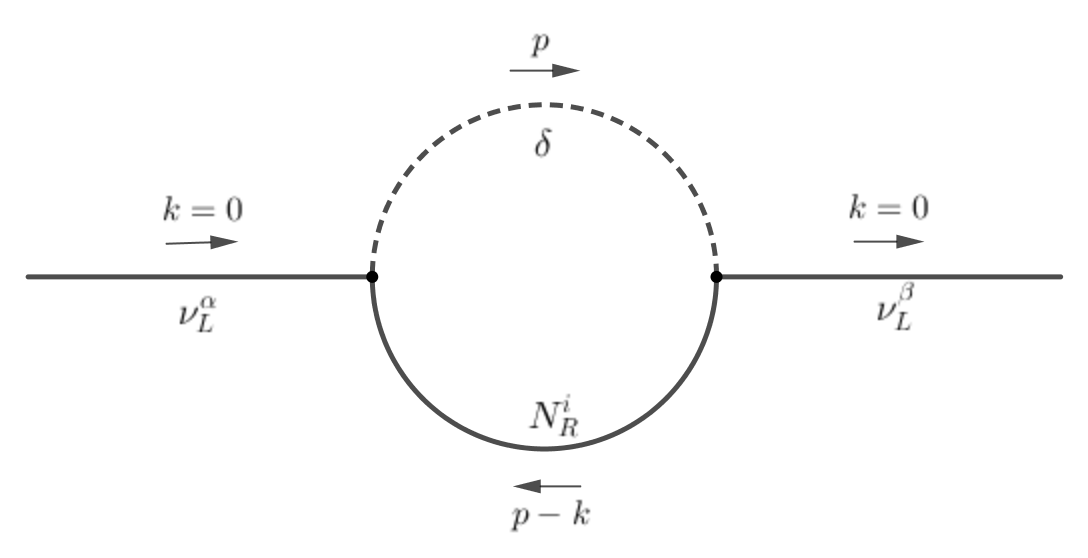
\includegraphics[width=0.7\linewidth]{oneloopreal}
  \caption{The one loop diagram contributing to the neutrino mass in the case that $\delta$ is a real scalar. The external neutrinos are evaluated at zero incoming momenta so as to extract only the mass contribution as opposed to the quadratic derivative interactions.}
  \label{fig:onelooprealdiag}
\end{figure}

\paragraph{Case 2: Complex Scalar Field}



To repeat the calculation for the complex scalar field, we should first think about the scalar degrees of freedom. Since the field is in the trivial representation of the electroweak gauge group, the most general hermitian mass term for $\delta$ can be written as \cite{Farzan2010};
\begin{equation}
  V_m = M^2 \delta^{\dagger} \delta - \frac{1}{2}(m^2 \delta\delta + \text{h.c.})
\end{equation}
Consider expanding the scalar field as $\delta = \tfrac{1}{\sqrt{2}}(\delta_1 + i\delta_2)$ where $\delta_{1,2}$ are both real fields. Expanding the terms above in terms of these real degrees of freedom;
\begin{dmath}
  V_m = \frac{1}{2}M^2(\delta_1 + i\delta_2)(\delta_1 - i\delta_2) - \frac{1}{4}m^2\left((\delta_1 + i\delta_2)(\delta_1 + i\delta_2) + (\delta_1 - i\delta_2)(\delta_1 - i\delta_2)\right)
\end{dmath}
Collecting the terms together for each field we find;
\begin{equation}
  V_m = \frac{1}{2}(M^2 - m^2)\delta_1^2 + \frac{1}{2}(M^2 + m^2)\delta_2^2
\end{equation}
We can then immediately see that the mass eigenstates are simply $\delta_1$ and $\delta_2$ themselves, with masses $m^2_{\delta_1} = M^2 - m^2$, $m^2_{\delta_2} = M^2 + m^2$. The lighter of these will be our Dark Matter candidate. Also note that interaction term \eqref{eq:effective lagrangian} is diagonal in this mass basis;
\begin{equation}
  \mathcal{L}_{\text{int}} = g_{i\alpha}\bar{N}^i_R \nu^\alpha_L (\delta_1 + i \delta_2)
\end{equation}
The contributions to the neutrino mass are then two diagrams of the form in Figure \ref{fig:onelooprealdiag}. One will have $\delta_1$ running round the loop, whilst the other will have $\delta_2$. We note that the only difference between them is that the second diagram will have two couplings with an extra factor of $i$, $(ig_{i\alpha})(ig_{i\beta}) = -g_{i\alpha}g_{i\beta}$. As such the second will come with a negative sign. The total contribution is then a sum of two contributions of the form \eqref{eq:oneloopmass result}. Importantly, we see that the dependence on the cutoff drops out in the complex case and we find;
\begin{equation}
  (m_\nu)_{\alpha\beta} = \sum_{i}{\frac{g_{i\alpha}g_{i\beta}}{16\pi^2}m_{N^i}\left(\frac{m_{\delta_2}^2}{m_{N^i}^2 - m_{\delta_2}^2}\log\frac{m_{N^i}^2}{m_{\delta_2}^2} - \frac{m_{\delta_1}^2}{m_{N^i}^2 - m_{\delta_1}^2}\log\frac{m_{N^i}^2}{m_{\delta_1}^2}\right)}
\end{equation}



\subsection{Why do we only have to worry about one process?}\label{sec:oneprocess}



In Section \ref{sec:crosssection} where we detailed how to do the calculation for $\nu\nu \rightarrow \delta\delta$, we neglected to calculate the cross section for other processes within the model that may also lead to a neutrino interaction. These additional processes are as follows;
\begin{enumerate}
  \item \textit{$\nu\nu \rightarrow NN$:} One can construct scenarios in parameter space where this dominates. However the centre of mass energy: $E_{\mathrm{com}} = \sqrt{2 E_\nu m_\nu}$ where $m_\nu$ is the mass of the cosmic neutrino background neutrino, is close to the mass of the lightest scalar $\delta$. By construction if the scalar is the dark matter candidate, then the mass of $N$, $m_N$, must be larger. Thus, even in scenarios where the centre of mass energy is large enough to produce two $N$ particles, the cross section is likely to lie at the front tail of the distribution and so be subdominant.
  \item $\nu N \rightarrow \nu N$: There is an $s$-channel and a $t$-channel diagram for this process. Independent of this however, we have assumed that $N$ is not the dark matter candidate. As such, we expect the relic density to be very low in comparison to all other particles. The vertex structure ensures that we expect the cross section to be of a similar order of magnitude to the $\nu\nu \rightarrow \delta\delta$ case. Hence, the contribution to the mean free path is negligible.
  \item $\nu\delta \rightarrow \nu\delta$: It is not immediately clear as to whether this will be negligible. Firstly, there is a $t$-channel process that will have a similar algebraic cross section as previously calculated in $\nu\nu \rightarrow \delta\delta$. There is also an $s$-channel process, whose cross-section we obtain from \cite{Franarin2018}. Secondly, we must check the contribution to the mean free path in two regimes;
  \begin{itemize}
    \item On a cosmological scale where $n_\delta$ is given by the relic density of dark matter,
    \item On a galactic scale, where the density is much higher within the dark matter halo.
  \end{itemize}
\end{enumerate}
Note that neglecting these processes is of course a simplifying assumption about the nature of the cross-sections, but they do not affect the interpretation of the results. This is because including any of the additional contributions above can only \textit{improve} the bounds; for a given $\ell$, introducing a new process increases the effective cross section, and reduces the mean free path leading to tighter constraints.

\subsection{Contribution from $\nu\delta \rightarrow \nu\delta$}
As mentioned above, we must check whether the $\nu\delta \rightarrow \nu\delta$ process contributes significantly to the mean free path of the blazar neutrino. In what follows, we will find that it does not contribute significantly. This is due to the fact that, even within the galactic halo, the cross-section is too small to generate a significant contribution.

\vspace{-0.5cm}

\subsubsection{$t$-Channel Cross Section}\label{sec:tchannel}

The relationship;
\begin{equation}
    u = m_\delta^2 - \frac{1}{2}s - \sqrt{s\left(\frac{1}{4}s - m_\delta^2\right)}\cos\theta
\end{equation}
along with the observation that for $\nu\delta \rightarrow \nu\delta$ with $m_\delta \sim \mO(\mathrm{MeV})$ and $E_\nu \sim \mO(TeV)$, it follows that $s \sim \mO(GeV) \gg m_\delta$. This then implies in this energy regime, $u \simeq s$. By crossing symmetry, we then deduce that the dependence of $\sigma_t(\nu\delta \rightarrow \nu\delta)$ on the centre of mass energy is just given by $\sigma(s)$ as in \eqref{eq:sigma}. To compare $\sigma(\nu\nu \rightarrow \delta \delta)$ and $\sigma_t(\nu\delta \rightarrow \nu\delta)$ we need only to evaluate $\sigma(s)$ at the different centre of mass energies, $s = 2E_\nu m_\nu$ and $s = 2 E_\nu m_\delta$. For an explicit comparison, we put in the values $g_e = 3 \times 10^{-3}$, $g_\mu = 10^{-2}$, $g_\tau = 3\times 10^{-1}$, $m_\delta = 0.5 \, \textrm{MeV}$, $m_\nu = 0.15 \, \textrm{eV}$, $m_N = 5\,\textrm{MeV}$. We find;
\begin{equation}
  \sigma(\nu\nu \rightarrow \delta\delta) \simeq 4.7\times 10^{-10} \, \textrm{MeV}^{-2}, \quad \sigma_t(\nu\delta \rightarrow \nu\delta) \simeq 6.2\times 10^{-16}\, \textrm{MeV}^{-2}
\end{equation}
So we find there is a difference of five to six orders of magnitude. After computing the number density of the dark matter in the galactic and cosmological cases, we will use this to deduce that the $t$-channel does not contribute.

\vspace{-0.5cm}

\subsubsection{$s$-Channel Cross Section}\label{sec:schannel}
We obtain an analytic expression for the $s$-channel cross-section from \cite{Franarin2018};
\begin{equation}
  \sigma_s(\nu_\mu\delta \rightarrow \nu_\ell \delta) = \frac{g_\mu^2 g_\ell^2}{16\pi}\frac{(m_N^2 - m_\delta^2)^2}{m_N^2 + m_\delta^2} \frac{1}{(s - m_N^2)^2 + \Gamma_N^2 m_N^2}
\end{equation}
where $\Gamma_N$ is the width of $N$, it is given by;
\begin{equation}\label{eq:sigma_s}
  \Gamma_N = \sum_{\ell}{\frac{g_\ell^2}{16\pi} \frac{(m_N^2 - m_\delta^2)^2}{m_N^3}}
\end{equation}
In this case, we simply do an order of magnitude estimate with;
\begin{equation}
  m_N = \mO(\textrm{MeV}), \quad m_\delta = \mO(\textrm{MeV}), \quad s - m_N^2 = \mO(\textrm{GeV}^2), \quad g = \mO(10^{-2})
\end{equation}
We note that this implies that $(s - m_N^2)^2 \gg \Gamma_N^2 m_N^2$. Putting these into \eqref{eq:sigma_s}, we find;
\begin{equation}
  \sigma_s(\nu\delta \rightarrow \nu\delta) \simeq \mO(10^{-21}\,\textrm{MeV}^{-2})
\end{equation}
As such we deduce that the contribution is certainly negligible at this energy, since even if the number density of $\delta$ was high enough, the $t$-channel process will dominate by $4$ or $5$ orders of magnitude. 

\subsubsection{The interference term}\label{sec:interference}
To argue that the interference term between the $s$ and the $t$ channel amplitudes, which we denote $\mM_s$ and $\mM_t$ respectively, also leads to a negligible contribution to the cross section, we note that by the triangle inequality;
\begin{equation}
    \Abs{\mM_s + \mM_t} \leq \Abs{\mM_s} + \Abs{\mM_t} \Rightarrow \Abs{\mM_s + \mM_t}^2 \leq \Abs{\mM_s}^2 + \Abs{\mM_t}^2 + 2\Abs{\mM_s}\Abs{\mM_t}
\end{equation}
Furthermore, integrals of these quantities which ultimately lead to the total cross section will satisfy equivalent relations due to the positive definite nature of the integrands. Finally then, if we denote the amplitude for $\nu\nu \rightarrow \delta\delta$ as $\mM$, the calculations in the previous two sections indicate that $\Abs{\mM_s}^2 \sim \mO(10^{-10})\Abs{\mM}^2$ and $\Abs{\mM_t}^2 \sim \mO(10^{-6})\Abs{\mM}^2$. Hence, by the triangle inequality, we deduce that $\Abs{\mM_s}\Abs{\mM_t} \sim \mO(10^{-8})\Abs{\mM}^2$ and therefore leads to a neglible contribution to the total squared amplitude, $\Abs{\mM_s + \mM_t}^2 \sim \Abs{\mM_t}^2 \sim \mO(10^{-6})\Abs{\mM}^2$. Hence we deduce that the total cross section for $\nu\delta \rightarrow \nu\delta$, where $\nu$ in the initial state has energy $\mO(\mathrm{TeV})$ satisfies $\sigma(\nu\delta \rightarrow \nu\delta) \sim 10^{-6} \cdot \sigma(\nu\nu\rightarrow \delta\delta)$. It therefore remains to check the number density of dark matter in the cosmological and galactic cases and compute the mean free path using the $t$-channel cross-section.

\subsubsection{Number Density on Cosmological Scales}
The dark matter density on a cosmological scale, at a redshift $z$, is given by \cite{Farzan2014};
\begin{equation}
  n(z) = \frac{\Omega_{\textrm{DM},0}\rho_c}{m_{\textrm{DM}}}(1 + z)^3 \simeq 1.26 \times 10^{-3} (1 + z)^3 \left(\frac{\textrm{MeV}}{m_{\textrm{DM}}}\right) \, \textrm{cm}^{-3}
\end{equation}
where we have used $\Omega_{\textrm{DM},0} \simeq 0.265$ and $\rho_c = 3H_0^2/8G \simeq 4.77\, \textrm{keV}\,\textrm{cm}^{-3}$. This is $5$ orders of magnitude below the cosmic neutrino background number density. So in order to be relevant, $\sigma(\nu\delta \rightarrow \nu\delta)$ would have to be approximately $10^5$ times larger than $\sigma(\nu\nu \rightarrow \delta\delta)$, evaluated at the neutrino energy. From Sections \ref{sec:tchannel}, \ref{sec:schannel}, and \ref{sec:interference}, we see this is not the case, and indeed the cross-section is significantly smaller than the $\nu\nu \rightarrow \delta\delta$ cross-section.  We can therefore neglect this cross section as the neutrino travels to the Milky Way.

\subsubsection{Number Density on Galactic Scales}
After deducing that the contribution to the mean free path from interaction with dark matter is negligible on cosmological scales, we just have to check whether the galactic overdesnity could lead to a significant contribution. As in \cite{Franarin2018}, we use the Einasto profile with $\alpha = 0.15$ and $R_0 = 20\,\textrm{kpc}$ to model the dark matter energy density;
\begin{equation}
  \rho_{\textrm{DM}}(r) = 7.2 \times 10^{-2}\,\textrm{GeV} \, \textrm{cm}^{-3}\, \cdot \exp\left(-\frac{2}{\alpha}\left(\left(\frac{r}{R_0}\right)^\alpha - 1\right)\right)
\end{equation}
We can obtain the number density by dividing by the mass of the dark matter particle, $m_\delta \simeq \mO(10^{-3} \, \textrm{GeV})$. Now, note that this is maximal when $r = 0$. In order to put an upper bound on the contribution to the optical depth, we assume that the whole halo has this maximal number density. With $m_\delta = 1\, \textrm{MeV}$;
\begin{equation}
  n_{\textrm{DM}}^{\textrm{max}} \simeq \frac{\rho_{\textrm{DM}}(r = 0)}{m_\delta} \simeq 4.4 \times 10^{7} \, \textrm{cm}^{-3} \simeq 10^{5} n^0_{\nu}
\end{equation}
Now we are in a position to see why this does not contribute to the suppression of the neutino flux from the blazar. Whilst the combination of $n^{\textrm{max}}_{\textrm{DM}} \sigma_t(\nu\delta\rightarrow\nu\delta)$ is now of the same order of magnitude as $n_\nu \sigma(\nu\nu\rightarrow \delta\delta)$, the relevant consideration is the probability that such an interaction ($\nu\delta \rightarrow \nu\delta$) occurs. This is dependent on the ratio between the length scale at which such a high number density is observed (i.e. the galactic radius), and the mean free path. Here, the mean free path, $\ell$, is $\mO(\textrm{Gpc})$, so the probability of survival is $\sim \exp(-d_{g}/\ell)$ where $d_g \simeq 1\,\textrm{kpc}$ is the galactic radius. We see that this is approximately unity. Finally, note that in the case where the mean free path is $\mO(\textrm{kpc})$, we would not expect the neutrino to reach anywhere close to the galaxy, so this would be inconsequential also. Hence we deduce that both in the cosmological and galactic settings, the contribution from $\nu\delta \rightarrow \nu\delta$ is negligible in comparison to the dominant $t$-channel process $\nu\nu \rightarrow \delta\delta$.

To end this section, we emphasise that whilst we have neglected the contribution from these other processes, including any/all of them can only improve the bounds as the mean free path will decrease with new interactions. As such, it is only for the sake of simplicity that we make the assumptions, \textit{not} at the cost of the validity of the bounds.



\subsection{Mass Splitting in the Complex Case}\label{sec:complexsplit}



We assume that each of the mass eigenstates is equally abundant $\nu_1, \bar{\nu}_1, \nu_2, \ldots$, with a number density given by;
\begin{equation}
  n_{\nu_i} = \frac{1}{6} n_\nu = \frac{1}{6} \cdot 340 \, \textrm{cm}^{-3}
\end{equation}
Now, the contribution from each mass eigenstate to the inverse mean free path $\ell^{-1}$ is given by $n_{\nu_i} \sigma(\nu_\mu X \rightarrow Y )$. Importantly we argued in the last section that we thus need only consider $\sigma(\nu_\mu \nu \rightarrow \delta \delta)$. Now, in the real case, there is nothing more to say as there is only one scalar mass eigenstate. In the complex case however, we must consider the following. The theory we are considering is effective up to some scale $\Lambda$. It therefore does not have to explicitly respect any of the symmetries that might apply in the UV. Indeed all we assume is that the new dark sector particles are odd under a $\mathbb{Z}_2$ symmetry, to ensure there is a stable candidate. As such, writing $\delta = \tfrac{1}{\sqrt{2}}(\delta_1 + i \delta_2)$, the most general hermitian mass term can be written;
\begin{equation}
  V_m = M^2 \delta\dagg \delta - \frac{1}{2}(m^2 \delta \delta + \textrm{h.c.})
\end{equation}
This leads to a mass splitting between the mass eigenstates $\delta_{1,2}$ given by $\Delta m_{12}^2 = 2m^2$. Now, we consider the possible processes $\nu\nu \rightarrow \textrm{scalars}$. We have;
\begin{equation*}
\nu\nu \rightarrow \delta_1 \delta_1, \quad \nu\nu \rightarrow \delta_1 \delta_2, \quad \nu\nu \rightarrow \delta_2 \delta_2
\end{equation*}
From this we see that there are a couple of scenarios that might occur kinematically. We assume that the lightest scalar is $\delta_1$, and that the first process can happen. Then it may the case that either (i) only the first process can occur, (ii) only the first and second processes can occur, or, (iii) all the processes can occur. This is where we make our simplifying assumption, which unlike the first case, will not necessarily improve the bounds if put in at a later date. We assume that if the first occurs, then the next two may also occur. This is equivalent to saying that there is a small mass gap between the two eigenstates. To simplify the situation then we assume that $m$ is small compared to $M$, and therefore that we can approximate;
\begin{equation}
  \sigma(\nu\nu \rightarrow \delta_1 \delta_1) + \sigma(\nu\nu \rightarrow \delta_1 \delta_2) + \sigma(\nu\nu \rightarrow \delta_2 \delta_2) \simeq 3 \sigma(\nu\nu \rightarrow \delta_1 \delta_1)
\end{equation}



\subsection{Redshift Considerations}



During the cosmological propagation, both the number density of the cosmic neutrino background neutrinos, and the energy of the blazar neutrino will be affected by redshift. Let the values now be denoted $n_\nu^0$ and $E_\nu^0$ respectively, then at a redshift $z$;
\begin{equation}
  n_\nu(z) = n_\nu^0 (1 + z)^3, \quad E_\nu(z) = (1 + z)E_\nu^0
\end{equation}
We now make the observation that the source of the $290 \, \textrm{TeV}$ neutrino is at a redshift $z = 0.3365$. In the case of the energy this means that the maximum possible multiplicative factor is $(1 + 0.3365)$, but this is within the confidence bounds on the energy measured at IceCube, so can be neglected. The redshift of the number density is not negligible however, although it only improves the bounds. We take the result from \cite{Farzan2014} that the optical depth is given by;
\begin{equation}
  \tau = c\int_{z = z_1}^{z = z_2}{\upd{z}\frac{\ud t}{\ud z}n(z)\sigma(z)}
\end{equation}
Now, the energy of the muon observed at IceCube had a 1$\sigma$ confidence interval of $23.7 \pm 2.8$ TeV \cite{IceCube2018}. This can be translated into an error on the energy of the incoming neutrino of an order 100 TeV. With this observation, we note that the energy of the 290 TeV neutrino at its source, i.e. before it is redshifted during the propagation, will lie within these bounds. Therefore, to simplify the analysis, we assume that $\sigma(z) = \sigma(E_\nu(z))$ does not depend on the redshift, $z$. With this assumption in mind, the expression above reduces to; 
\begin{equation}
  \tau = c n_\nu^0 \sigma(E_\nu^0) \int_{z = z_1}^{z = z_2}{\upd{z}(1 + z)^3 \frac{\ud t}{\ud z}}
\end{equation}
We can relate $\ud t/\ud z$ to the Hubble rate via;
\begin{equation}
  \frac{\ud t}{\ud z} = -\frac{1}{(1 + z)H(z)}
\end{equation}
where;
\begin{equation}
  H(z) = H_0 \sqrt{\Omega_\Lambda + \Omega_{m,0}(1 + z)^3}
\end{equation}
We will take the values $\Omega_\Lambda \simeq 0.65$, $\Omega_{m,0} \simeq 0.315$, $H_0 \simeq 6.73 \times 10^{4}\, \textrm{km}\,\textrm{s}^{-1}\textrm{Gpc}^{-1}$ \cite{Planck}, $c = 3\times 10^{5}\,\textrm{km s}^{-1}$. Letting $\ell_0^{-1} := n_\nu^0 \sigma(E_\nu^0)$ to find;
\begin{equation}
  \tau = \left(\frac{\ell_0}{\text{Gpc}}\right)^{-1} \left(\frac{c \, / \, \text{km s}^{-1}}{H_0 \, /\, \text{km s}^{-1}\text{Gpc}^{-1}}\right) \cdot \int_{z = z_1}^{z = z_2}{\upd{z}\frac{(1 + z)^2}{\sqrt{\Omega_\Lambda + \Omega_{m,0}(1 + z)^3}}} \simeq 1.90 \left(\frac{\ell_0}{\textrm{Gpc}}\right)^{-1}
\end{equation}


\subsection{Including Neutrino Mass Hierarchies}


The last technicality to introduce into the computation of the bounds are the facts that;
\begin{enumerate}
  \item The neutrino \textit{mass} eigenstates and \textit{flavour} eigenstates are not the same
  \item The neutrino masses are unknown, and indeed have two possible orderings (for the mass eigenstates); the \textit{normal hierarchy} and the \textit{inverted hierarchy}.
\end{enumerate}
Within our calculation we aim to present the situation for both of these cases.

\subsubsection{Mass Eigenstates and the PMNS Matrix}

Within the Standard Model, we expect neutrinos to be massless. Experiments illustrating phenomena such as neutrino oscillations contradict this fact and we now believe they do indeed have a small mass. This complicates matters however for the reason mentioned above. The flavour eigenstates and the mass eigenstates are no longer the same in this case. Instead they are related by the \textit{PMNS} matrix\footnote{Pontecorvo-Maki-Nakagawa-Sakata}. This encodes a unitary transformation between the flavour basis and the mass basis:
\begin{equation}
\nu_\ell := \begin{pmatrix} \nu_e \\ \nu_\mu \\ \nu_\tau \end{pmatrix} = \thrbythr{U_{e1} & U_{e2} & U_{e3}}{U_{\mu1} & U_{\mu2} & U_{\mu3}}{U_{\tau1} & U_{\tau2} & U_{\tau3}} := U \nu_i
\end{equation}

\subsubsection{The Mass Hierarchy}

A key fact in this discussion is that ultimately we do not know the absolute values, nor the ordering of the mass eigenstates. There are two common alternatives, which are illustrated in Figure 2 in \cite{King};
\begin{enumerate}
  \item \textit{Normal Ordering:} In the normal hierarchy, $\nu_3$ is the most massive state, whilst $\nu_1$ and $\nu_2$ are lighter.
  \item \textit{Inverted Ordering:} On the other hand, in the inverted case, $\nu_3$ is the lightest, whilst $\nu_1$ and $\nu_2$ are heavier.
\end{enumerate}

\subsubsection{Constraints on the Masses}

We can go slightly further, whilst we do not know the precise masses of the neutrinos we have (i) a bound on the total sum of the masses that comes from Cosmology, and, (ii) values for the mass difference between the eigenstates. To be more precise;
\begin{itemize}
  \item Combining constraints from Cosmic Microwave Background (CMB) anisotropies, Baryon Acoustic Oscillations, Type 1A Supernovae, and, CMB lensing, we will use the constraint \cite{Couchot2017};
  \begin{equation}
    \sum{m_{\nu_i}} < 0.17 \, \textrm{eV}
  \end{equation}
  \item We also know the squared mass differences between some of the mass eigenstates \cite{Couchot2017};
  \begin{align}
    \Delta m_{12}^2 = m_2^2 - m_1^2 &= 7.37 \times 10^{-5}\,\textrm{eV}^2 \\
    \Delta m^2 = m_3^2 - \frac{1}{2}(m_1^2 + m_2^2) &= +2.50 \times 10^{-3} \, \textrm{eV}^2\, \textrm{(NH)} \\
    &= -2.46 \times 10^{-3} \, \textrm{eV}^2\, \textrm{(IH)}
  \end{align}
\end{itemize}
From the last of these constraints we see that fixing one of the masses automatically fixes the others. In our analysis we intend to vary one of the masses of the mass eigenstates and use the squared mass differences to compute the other masses, remaining within the bound set by the cosmological considerations. We will present the analysis in both the normal and inverted cases.


\subsection{The Coupling Constants}


There is one final consequence of the non-coincidence of the mass and flavour eigenstates. We are considering a coupling in the Lagrangian of the form;
\begin{equation}
  \mL_{\textrm{new}} = \sum_{\ell}{g_\ell \delta \bar{N}_R \nu_{\ell, L} + \textrm{h.c.}}
\end{equation}
where importantly, the $\nu_{\ell}$ are the flavour eigenstates. Furthermore, we quoted constraints on the couplings $g_\ell$ in this flavour basis e.g. $g_{\ell} < 10^{-3}$ in the case of real dark matter. Now consider expanding in the mass basis;
\begin{equation}
  \mL = \delta \bar{N}_R \sum_{\ell}{g_\ell \sum_{i}{U_{\ell i}\nu_{i, L}}} + \textrm{h.c.} := \sum_i{g_i \delta \bar{N}_R \nu_{i, L}}
\end{equation}
We have defined the couplings to the neutrino mass eigenstates;
\begin{equation}
  g_i := \sum_{\ell}{U_{\ell i}g_{\ell}}
\end{equation}
Now, importantly, these will inherit constraints from the constraints on the flavour basis couplings, and are just related by a linear transformation. This means that we can still parametrise our constraints in terms of the flavour couplings. The context of these comments is that the cosmic neutrino background consists of decoherent mass eigenstates. Therefore instead of considering flavour processes $\nu_\mu \nu_\ell, \nu_\mu \bar{\nu}_\ell \rightarrow \delta\delta$, we should instead consider $\nu_\mu \nu_i \rightarrow \delta \delta$. To do so we should use the $\set{g_i}$ couplings at the $\nu_i \delta N$ vertex, which we can compute as above. We also make use of the mass eigenstate masses as discussed above to compute the centre of mass energy in each of the different cases $i = 1,2,3$. Finally, we will assume that each of the mass eigenstates is equally abundant in the cosmic neutrino background so that we can take the number density of each species to be $n_\nu/6$ as noted previously.

\subsection{Neutrino Clustering}


This is the phenomenon relating to the gravitational clustering of neutrinos at late times once they become non-relativistic. This can increase their density inside gravitational wells such as the Milky Way today.  An important reference is \cite{Ringwald2004} which discusses the clustering of cosmic neutrino background neutrinos onto cold dark matter. In the context of this work, this would affect the number density $n_\nu(z)$ as the astrophysical neutrino passed through different dark matter distributions. In regions where there is more cold dark matter, \cite{Ringwald2004} suggests that we should also see more cosmic neutrino background neutrinos. A precision analysis of the propagation of the neutrinos from the blazar should take this into account.

This being said, \cite{Ringwald2004} only extends the analysis to the local group\footnote{The \textit{Greisen-Zatsepin-Kuzmin} zone}, across distances of $\textrm{Mpc}$. This is ultimately small scale structure in the context of $\textrm{Gpc}$ propagation. Figure 8 in \cite{Ringwald2004} illustrates the density contrast of the neutrinos on this scale. We see that density constrasts of $\mO(2)$ are realistic, so including this effect could strengthen the bounds. Even an increase of an order of magnitude within the local group would only change the optical depth at the percent level, so we neglect this effect in this work.

\begin{figure}[t]
 \centering
 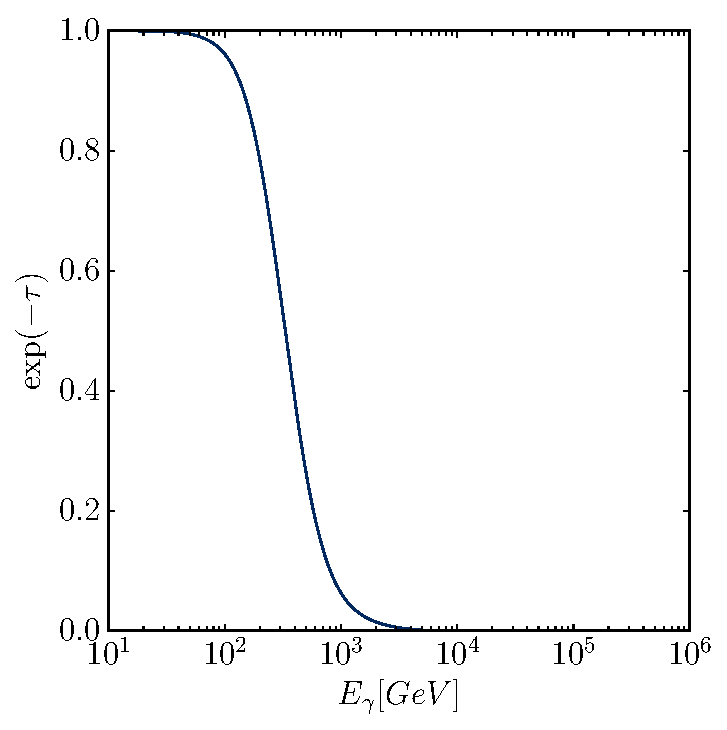
\includegraphics[width=.5\textwidth]{ebl.pdf}
 \caption{The probability, $\exp(-\tau)$, where $\tau$ is the optical depth, of a photon produced in the blazar jet reaching the Earth due to interactions with the EBL. We see that at Fermi-LAT energies, $\mO(290) \, \mathrm{GeV}$, this probability is close to 1, whilst at the higher, HAWC energies, $\mO(1 - 100) \, \mathrm{TeV}$, there is significant attenuation of the flux due to scatterings $\gamma\gamma \rightarrow e^{+}e^{-}$. These calculations are based on \cite{DeLavallaz:2011ju}.}
 \label{fig:ebl}
\end{figure}

\subsection{Discussion regarding the consistency of the neutrino and photon flux}\label{sec:consistent}

In this subsection we would like to discuss the neutrino flux we use above and see how it compares to the observed photon flux.  The discussion here is a simple sanity check, this subsection therefore on its own contains no results which have any impact on the bound we obtain later. In particular, we are not using the photon flux to derive a bound, we just aim to discuss the discrepancy between the two fluxes.

Let us recall how neutrinos and photons are thought to be generated in the relativistic jets of active galaxies. In the hadronic scenario, highly boosted protons interact with photons in the jet from e.g. electron synchotron radiation. This leads to the production of neutral and charged pions via resonances (for example $p\gamma \rightarrow \Delta^+ \rightarrow p\pi^0$) or direct production (for example $p\gamma \rightarrow n\pi^+$). These highly relativistic pions then decay via $\pi^0 \rightarrow \gamma \gamma$ and $\pi^+ \rightarrow \ell^+ \nu_\ell$ where $\ell$ is a lepton \cite{Mucke:1998mk, Szabo:1994qx}. This leads to a production of neutrinos and photons with $F_\nu \sim F_\gamma$ within the jet \cite{Keivani2018}. We might expect that the detection of high energy neutrinos should thus be accompanied by the EM emission of pionic gamma-rays. If this were the case, we would indeed expect the luminosities of the neutrinos and the photons to be comparable, $F_\nu \sim F_\gamma$, as was assumed in \cite{Kelly}.  Unlike the HAWC constraint, the Fermi-LAT data consisted of an actual measurement, and those authors used this assumption to make a direct prediction for the neutrino flux.

The assumption that $F_\nu \sim F_\gamma$ is however conservative --- since the neutrinos are weakly interacting, they escape the jet without attenuation to the flux. On the other hand, the photons produced by neutral pion decays, may \textit{not} be observed due to electromagnetic processes which may occur in the jet or attenuation during propagation across on the Universe. In the latter case this is due to $\gamma\gamma \rightarrow e^+ e^-$ attentuation on the Extragalactic Background Light (EBL) \cite{Finke:2009xi}.  In Figure \ref{fig:ebl} we use code developed by one of the authors for a previous project \cite{DeLavallaz:2011ju} to show the attentuation due to pair production on the EBL for high energy photons from a blazar at redshift $z=0.34$ is not very important at the Fermi-LAT energies considered in \cite{Kelly} ($<$ 290 GeV) but really cuts off the photon flux at the HAWC energies relevant here (0.8 TeV --- 74 TeV). Because of this, the HAWC data acting as an upper bound is in no conflict with the jet physics.

The HAWC data in Table \ref{tab:luminosity} shows that the photon flux at this energy is less than the neutrino flux we have assumed.  Given the fact it is much easier for photons to be attenuated and to lose energy than neutrinos, we assume this is in fact what has happened and note that we have assumed the lower of the two possible estimates of the neutrino flux based on the observed event.